% !Mode:: "TeX:UTF-8"
% !TEX program  = xelatex
% !BIB program  = biber
\documentclass[AutoFakeBold,AutoFakeSlant,scheme=chinese,degree=bachelor,zihao=-4]{sustechthesis}
% 1. AutoFakeBold 与 AutoFakeSlant 为伪粗与伪斜,如果本机上有相应粗体与斜体字体,请使用 xeCJK 宏包进行设置,例如:
%   \setCJKmainfont[
%     UprightFont = * Light,
%     BoldFont = * Bold,
%     ItalicFont = Kaiti SC,
%     BoldItalicFont = Kaiti SC Bold,
%   ]{Songti SC}
%
% 2. scheme=chinese 为 ctexart 文类提供的中文排版方案,如果使用英文进行论文创作,请使用 scheme=plain 选项。
%
% 3. degree=bachelor 为 sustechthesis 文类提供的本科生毕业论文模板,其他可选项为 master 与 doctor,但是均未实现,如果您对此有兴趣,欢迎 PR。
%
% 4. sustechthesis.cls 文类主要参考自去年完成使命的 sustechthesis.tex,在这一年的时间,作者的 TeX 风格与常用宏包发生许多变化,因为之前的思想为仅提供必要的格式修改相关代码,所以转换为文类形式所进行的修改较少,而近期的风格与常用宏包均体现在以下的例子文件中。
%
% 5. 示例文件均放置于相应目录的 examples 文件夹下,构建自己论文时可暂时保留,用以检索接口与使用方法。
%
% 6. 英文目录需要居中可以使用:\renewcommand{\contentsname}{\centerline{Content}}
%
% 7. LaTeX 中公式编号括号样式及章节关联的方法:https://liam.page/2013/08/23/LaTeX-Formula-Number/

% !Mode:: "TeX:UTF-8"
% !TEX program  = xelatex

% 数学符号与环境
\usepackage{amsmath,amssymb}
  \newcommand{\dd}{\mathrm{d}}
  \newcommand{\RR}{\mathbb{R}}
% 参考文献
\usepackage[style=gb7714-2015]{biblatex}
  \addbibresource{ref.bib}
% 无意义文本
\usepackage{zhlipsum,lipsum}
% 列表环境设置
\usepackage{enumitem}
% 浮动题不越过 \section
\usepackage[section]{placeins}
% 超链接
\usepackage{hyperref}
% 图片,子图,浮动题设置
\usepackage{graphicx,subcaption,float}
% 抄录环境设置,更多有趣例子请命令行输入 `texdoc tcolorbox`
\usepackage{tcolorbox}
  \tcbuselibrary{xparse}
  \DeclareTotalTCBox{\verbbox}{ O{green} v !O{} }%
    {fontupper=\ttfamily,nobeforeafter,tcbox raise base,%
    arc=0pt,outer arc=0pt,top=0pt,bottom=0pt,left=0mm,%
    right=0mm,leftrule=0pt,rightrule=0pt,toprule=0.3mm,%
    bottomrule=0.3mm,boxsep=0.5mm,bottomrule=0.3mm,boxsep=0.5mm,%
    colback=#1!10!white,colframe=#1!50!black,#3}{#2}%
\tcbuselibrary{listings,breakable}
  \newtcbinputlisting{\Python}[2]{
    listing options={language=Python,numbers=left,numberstyle=\tiny,
      breaklines,commentstyle=\color{white!50!black}\textit},
    title=\texttt{#1},listing only,breakable,
    left=6mm,right=6mm,top=2mm,bottom=2mm,listing file={#2}}
% 三线表支持
\usepackage{booktabs}

% LaTeX logo
\usepackage{hologo}
 % 导言区
% !Mode:: "TeX:UTF-8"
% !TEX program  = xelatex
\设置信息{
    % 键 = {{中文值}, {英文值}},
    分类号 = {{}, {}},
    编号 = {{}, {}},
    UDC = {{}, {}},
    密级 = {{}, {}},
    % 仅题目(不含副标题)、系别、专业,支持手动 \\ 换行,不支持自动换行。
    题目 = {{南方科技大学毕业论文模板设计\\\hologo{LaTeX} 形式 v\version}, {Graduation Thesis Template\\\hologo{LaTeX} Format v\version}},
    % 如无需副标题,删除值内容即可,不可删除键定义。
    副标题 = {{副标题}, {Sub-title}},
    姓名 = {{梁钰栋}, {Iydon Liang}},
    学号 = {{11711217}, {11711217}},
    系别 = {{数学系}, {Department of Mathematics}},
    专业 = {{信息与计算科学}, {Computatoinal Mathematics}},
    指导老师 = {{高德纳}, {Donald~E.~Knuth}},
    时间 = {{2019年12月8日}, {December 8, 2019}},
    职称 = {{教授}, {Professor}},
}
 % 论文信息
\begin{document}

\中文标题页\英文标题页
\中文诚信承诺书\英文诚信承诺书
\摘要标题
% !Mode:: "TeX:UTF-8"
% !TEX program  = xelatex
\begin{中文摘要}{\LaTeX ;接口}
  笔者见到的毕业论文模板,大多是以文类的形式,少部分以宏包的形式,并且在模板中大多掺杂着各式各样的例子(除了维护频率高的模板),导致模板文件使用了大部分与形式格式不相关的内容,代码量巨大文档欠缺且不容易修改,出现问题需要查看宏包或者文类的源代码。于是,秉着仅提供实现最基本要求的理念,重构了之前所写的 \TeX\ 形式。由于第二年使用该模板,所以设计出的模板接口不能保证以后不发生重大变动,一切以文档为主。毕竟学校在发展初期,各类文件都在日渐完善,前几年时,学校标志及名称还发生变化,同时毕业论文的样式也发生了重大变化。但是可以保证的是,模板提供的接口均为中文形式\footnote{使用 \hologo{XeLaTeX} 特性,一方面增加辨识度,另一方面不拘泥于英文命名的规则。当然此举也有些许弊端,在此就不过多展开。},并且至少更新到 2021 年,也就是笔者毕业。模板这种东西不能保证一劳永逸,一方面学校的标准制度都在发生着改变,另一方面 \hologo{LaTeX} 的宏包也在发生着改变,早先流行的宏包可能几年后就被“淘汰”掉。因此,您的使用与反馈是我不断更新的动力,希望各位不吝赐教。
\end{中文摘要}

\begin{英文摘要}{LaTeX, Interface}
  \lipsum[1]
\end{英文摘要}
 % 论文摘要

\目录\clearpage % 目录及换页

% !Mode:: "TeX:UTF-8"
% !TEX program  = xelatex
\section{免责声明}
\begin{enumerate}[label={\alph*)}]
    \item 本模板的发布遵守 \LaTeX\ Project Public License,使用前请认真阅读协议内容。
    \item 南方科技大学教学工作部只提供毕业论文写作指南,不提供官方模板,也不会授权第三方模板为官方模板,所以此模板仅为写作指南的参考实现,不保证格式审查老师不提意见. 任何由于使用本模板而引起的论文格式审查问题均与本模板作者无关。
    \item 任何个人或组织以本模板为基础进行修改,扩展而生成的新的专用模板,请严格遵守 \LaTeX\ Project Public License 协议。由于违犯协议而引起的任何纠纷争端均与本模板作者无关。
\end{enumerate}

% !Mode:: "TeX:UTF-8"
% !TEX program  = xelatex
\section{文类接口}
文类的接口的命名均为汉字,意思为字面意思,如有疑问,欢迎在 GitHub 提出 \href{https://github.com/Iydon/sustechthesis/issues}{Issues}。

\subsection{汉化字号接口}
本接口主要使用 \texttt{ctex} 宏包。

\verbbox{\初号},\verbbox{\小初},\verbbox{\一号},\verbbox{\小一},\verbbox{\二号},\verbbox{\小二},\verbbox{\三号},\verbbox{\小三},\verbbox{\四号},\verbbox{\小四},\verbbox{\五号},\verbbox{\小五},\verbbox{\六号},\verbbox{\小六},\verbbox{\七号},\verbbox{\八号}。


\subsection{汉化字体接口}
可能本机上部分字体不存在,导致部分字体无法使用。

\verbbox{\宋体},\verbbox{\黑体},\verbbox{\仿宋},\verbbox{\楷书},\verbbox{\隶书},\verbbox{\幼圆},\verbbox{\雅黑},\verbbox{\苹方}。


\subsection{字体效果接口}

建议在正文时使用 \verb|\textbf{}|,\verb|\textit{}| 调用\textbf{粗体}与\textit{斜体}。

It is recommended to use \verb|\textbf{}|,\verb|\textit{}| to call \textbf{Bold} and \textit{ItalicFont}.

\verbbox{\粗体},\verbbox{\斜体}。


\subsection{格式相关接口}
\subsubsection{命令}
例子请参考前文,在写论文初期,可以注释掉标题页等不必要信息,以加快编译速度。

\verbbox{\设置信息},\verbbox{\目录},\verbbox{\下划线},\verbbox{\中文标题页},\verbbox{\英文标题页},\verbbox{\中文诚信承诺书},\verbbox{\英文诚信承诺书},\verbbox{\摘要标题},\verbbox{\参考文献},\verbbox{\附录},\verbbox{\致谢}。

\subsubsection{环境}
摘要环境均需一个参数,为关键词:\verb|\begin{}{}...\end{}|。

\verbbox{中文摘要},\verbbox{英文摘要}。

% !Mode:: "TeX:UTF-8"
% !TEX program  = xelatex

\section{一些样例}

\subsection{表格}

\begin{table}[htb]
% h-here,t-top,b-bottom,优先级依次下降
    \begin{center}
    % 居中
        \caption{表格的标题应该放在上方}\label{table}
        \begin{tabular}{lc} % 三线表不能有竖线,l-left,c-center,r-right
            \toprule
            %三线表-top 线
            Example & Result \\
            \midrule
            %三线表-middle 线
            Example1          & 0.25 \\
            Example2          & 0.36 \\
            \bottomrule
            %三线表-底线
        \end{tabular}
    \end{center}
\end{table}

\subsection{参考文献}

参考文献如是\cite{Nicholas1998Handbook}。

\begin{figure}[htb]
    \centering
    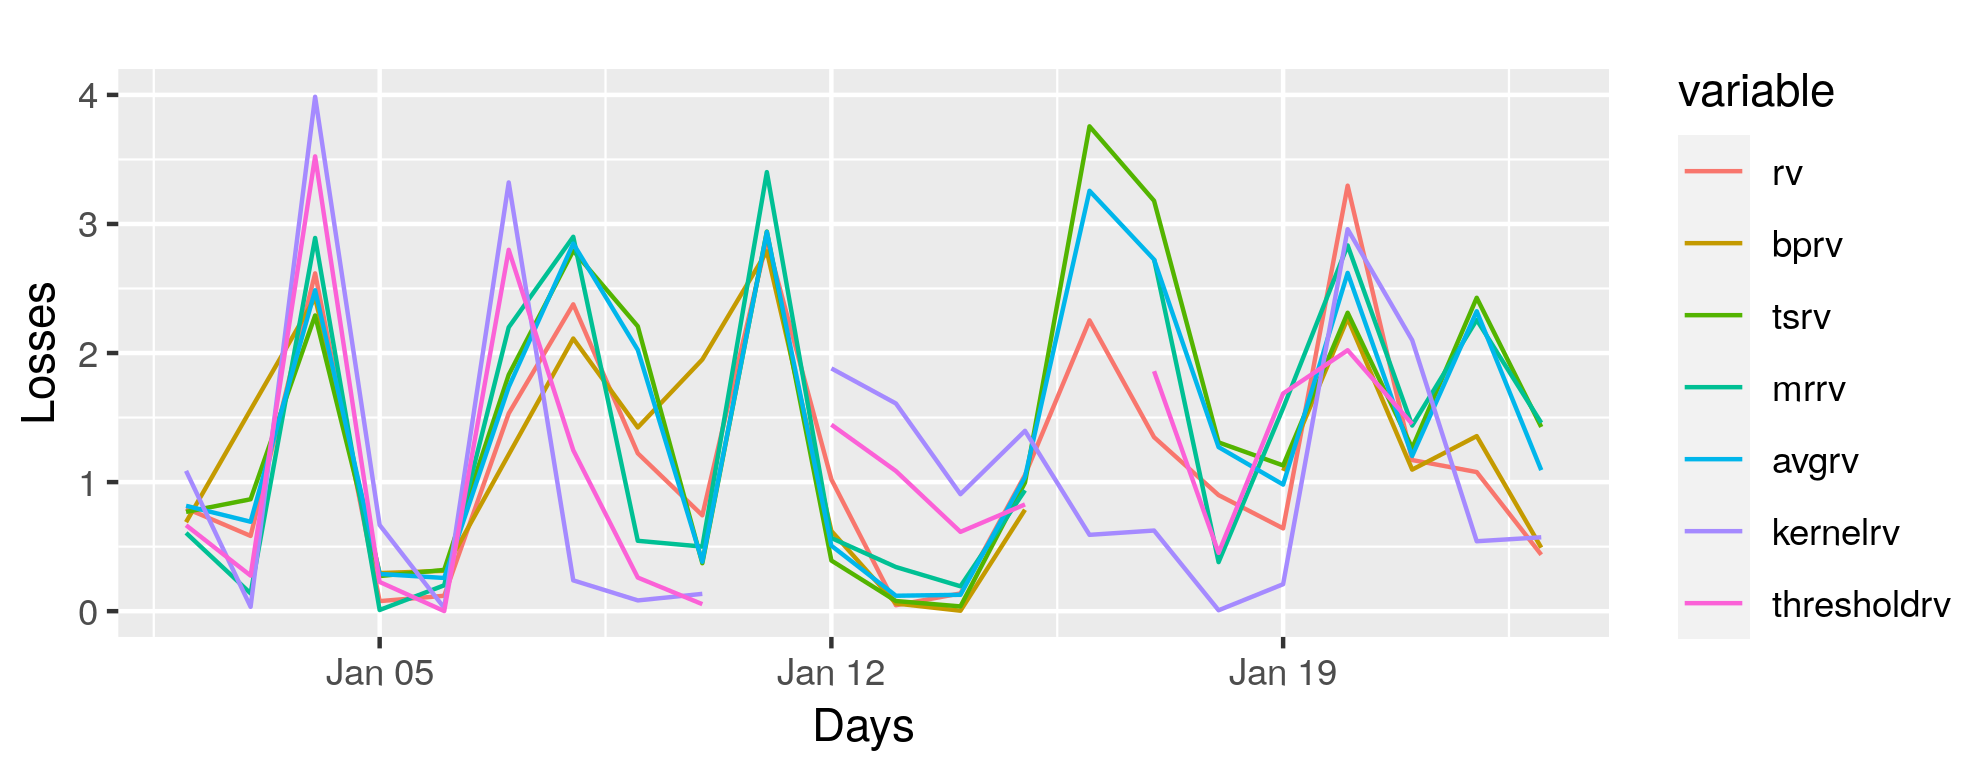
\includegraphics[width=.5\textwidth]{example-image-a}
    \caption{自带测试图片---Test image}\label{F:test-a}
    % 图片的标题应该在下方
\end{figure}

\begin{figure}[htb]
    \centering
    \begin{subfigure}[t]{.45\linewidth}
        \centering
        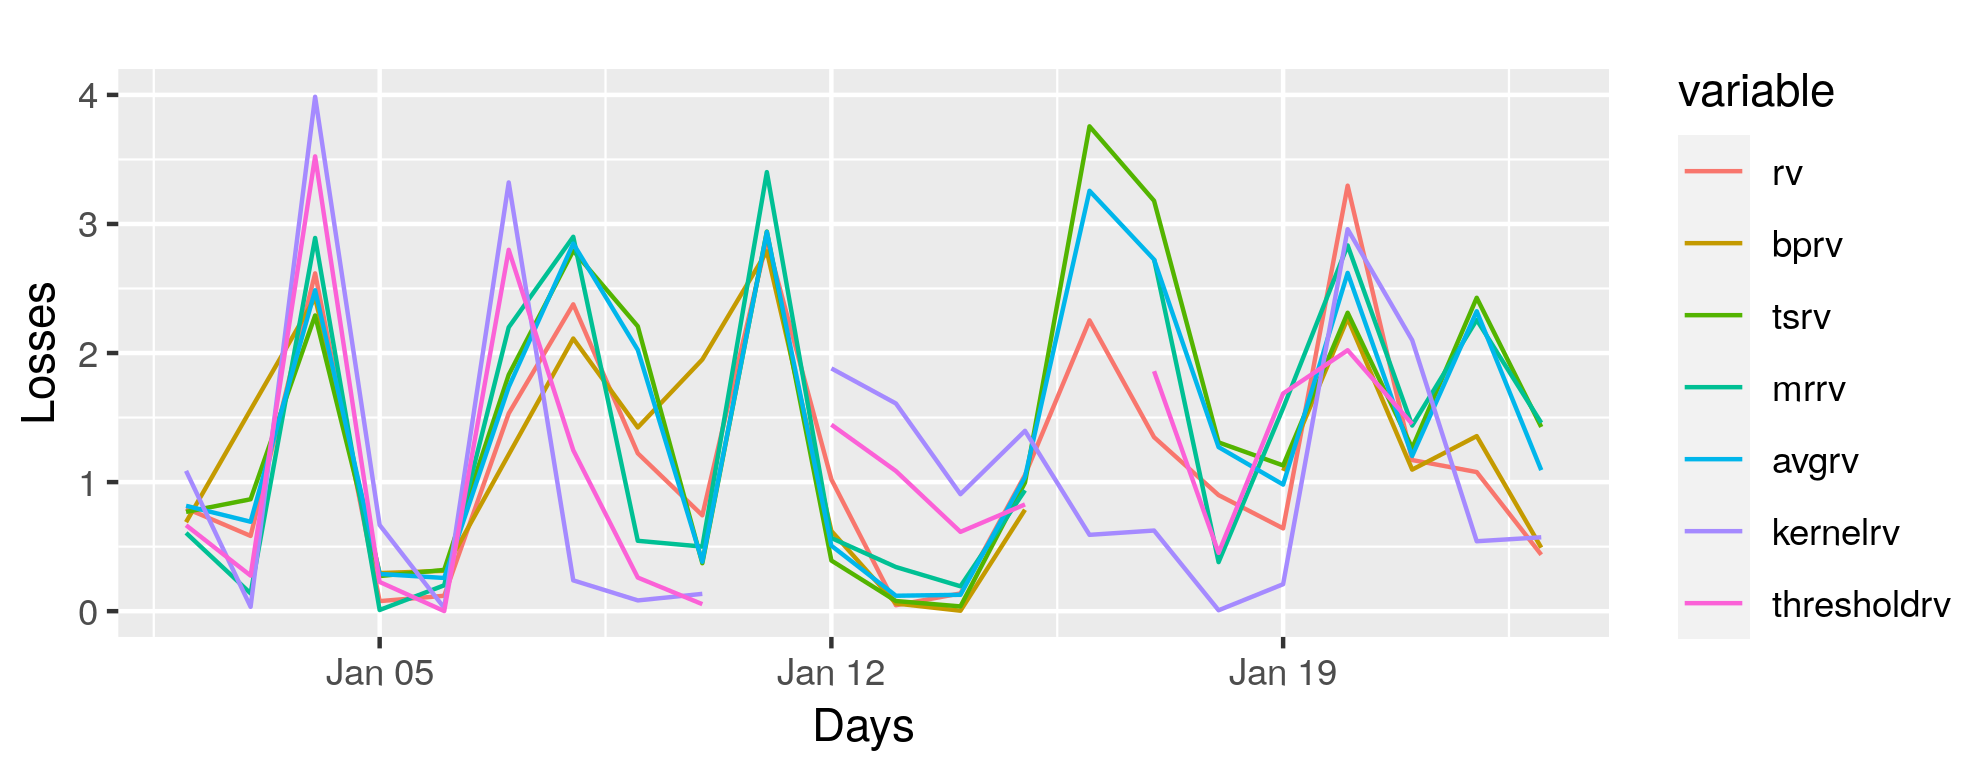
\includegraphics[width=1\textwidth]{example-image-a}
        \caption{子图-自带测试图片---Test image}\label{F:test-b-sub-a}
    \end{subfigure}
    \begin{subfigure}[t]{.45\linewidth}
        \centering
        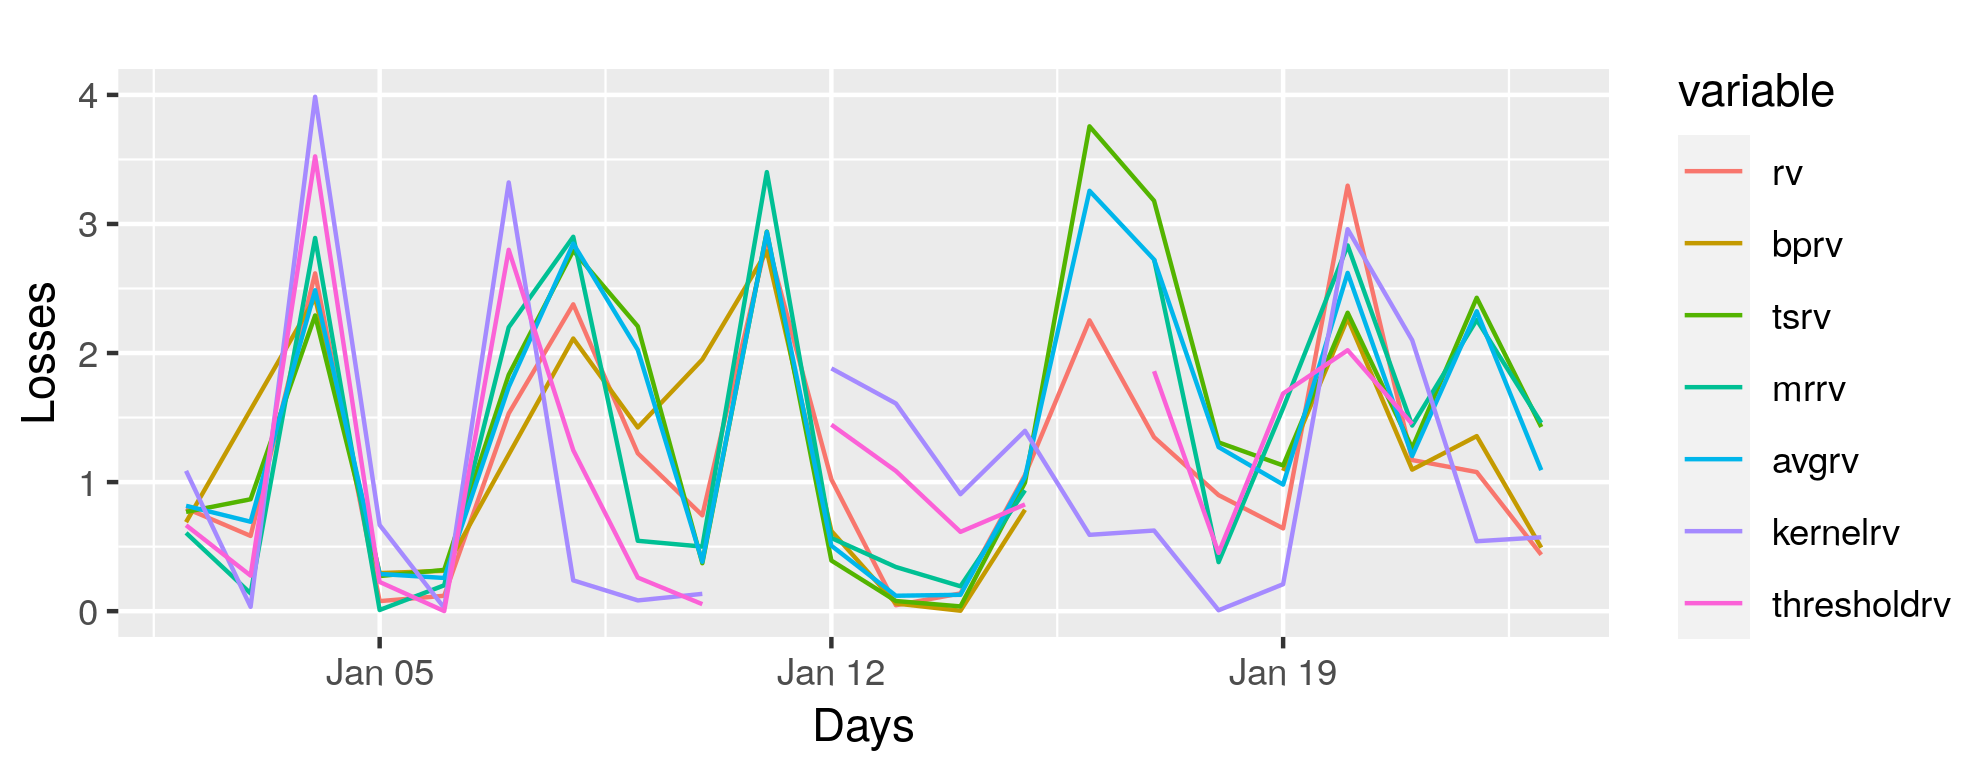
\includegraphics[width=1\textwidth]{example-image-a}
        \caption{子图-自带测试图片---Test image}\label{F:test-b-sub-b}
    \end{subfigure}
    \caption{自带测试图片---Test image}\label{F:test-b}
\end{figure}
% !Mode:: "TeX:UTF-8"
% !TEX program  = xelatex
\section{\LaTeX\ 入门}
请参考 \href{https://tex.readthedocs.io/zh_CN/latest/}{在线文档},包括学习资源及学习路径。欢迎在 GitHub 上提出 \href{https://github.com/Iydon/tex/issues}{Issues}。
\clearpage
\参考文献
  \printbibliography[heading=none]\clearpage
\附录
  % !Mode:: "TeX:UTF-8"
% !TEX program  = xelatex
\section*{数据获取函数}\label{A:data}
\Python{utils.py}{code/examples/utils.py}
\clearpage
\致谢
  % !Mode:: "TeX:UTF-8"
% !TEX program  = xelatex
\sustechthesis\ 目前版本为 \version, \LaTeX\ 毕业论文模板项目从提出到现在已有两年了。感谢为本项目贡献代码的开发人员们:
\begin{itemize}
    \item 梁钰栋(南方科技大学,本科 17 级);
    \item 张志炅(南方科技大学,本科 17 级)。
\end{itemize}
以及使用本项目,并提出诸多宝贵的修改意见的使用人员们:
\begin{itemize}
    \item 李未晏(南方科技大学,本科 15 级);
    \item 张尔聪(南方科技大学,本科 15 级)。
\end{itemize}

此外,目前的维护者并非计算机系,可能存在对协议等的错误使用,如果你在本模板中发现任何问题,请在 GitHub 中提出 \href{https://github.com/Iydon/sustechthesis/issues}{Issues},同时也非常欢迎对代码的贡献!

\end{document}
